\documentclass[12pt]{article}
 \usepackage[margin=1in]{geometry}
\usepackage{amsmath,amsthm,amssymb,amsfonts,listings,graphicx,appendix,float}

\usepackage[utf8]{inputenc}
\DeclareUnicodeCharacter{3000}{-}%
\newcommand{\N}{\mathbb{N}}
\newcommand{\Z}{\mathbb{Z}}

\newenvironment{problem}[2][Problem]{\begin{trivlist}
\item[\hskip \labelsep {\bfseries #1}\hskip \labelsep {\bfseries #2.}]}{\end{trivlist}}
%If you want to title your bold things something different just make another thing exactly like this but replace "problem" with the name of the thing you want, like theorem or lemma or whatever

\begin{document}

%\renewcommand{\qedsymbol}{\filledbox}
%Good resources for looking up how to do stuff:
%Binary operators: http://www.access2science.com/latex/Binary.html
%General help: http://en.wikibooks.org/wiki/LaTeX/Mathematics
%Or just google stuff

\title{CSE417 homework 1}
\author{Muzhou Liu }
\date{September 12, 2018}
\maketitle


\begin{enumerate}
\item LDF problem 1.3 Prove that the PLA eventually converges to a linear separator for separable data. The following steps will guide you through the proof. Let $w^{*}$ be an optimal set of weights (one which separates the data). The essential idea in this proof is to show that the PLA weights $w(t)$ get “more aligned” with $w^{*}$ with every iteration. For simplicity, assume that $w(0) = 0$.
    \begin{enumerate}
      \item Let  $\rho = \min_{1 \leq n \leq N} {y_{n}(w^{*T}x_{n})}$. Show that $\rho > 0$.
        Because all x(t) are correctly classified by w(t) so:
        \begin{itemize}
          \item $y(t) = + 1: sign(w^{T}(t)x(t)) = + 1 \Leftrightarrow w^{T}(t)x(t) > 0$. \\ Thus:$ y(t)w^{T}(t)x(t) > 0$.
          \item $y(t) = - 1: sign(w^{T}(t)x(t)) = - 1 \Leftrightarrow w^{T}(t)x(t) > 0$. \\ Thus:$ y(t)w^{T}(t)x(t) > 0$.
          Therefore, as minimum value of $y(t)w^{T}(t)x(t) $ ,$\rho$ must larger than 0.
        \end{itemize}
      \item Show that $w^{T}(t)w^{*} \geq w^{T}(t-1)w^{*}+\rho$, and conclude that $ w^{T}(t)w^{*} \geq t\rho$ \\
      \begin{proof}
      Because we have  \begin{equation*}
                         w^{T}(t - 1) = (w(t) - y(t)x(t))^{T} = w^{T}(t) - y(t)x^{T}(t)
                       \end{equation*}
      $\Leftrightarrow  w^{T}(t-1)w^{*}+\rho = w^{T}(t)w^{*} - y(t)x^{T}(t)w^{*} + \rho $ \\
      According to the definition of $\rho$ We also have: $\rho \leq y(t)x^{T}(t)w^{*}$ (as proved in part (a)), which means: $\rho - y(t)x^{T}(t)w^{*} \leq 0$. \\
      Then: \\
      $ w^{T}(t)w^{*} - y(t)x^{T}(t)w^{*} + \rho \leq w^{T}(t)w^{*} $ \\ \\

        Base case: when $t = 0$: $w^{T}(0)w^{*} \geq 0\rho \Leftrightarrow 0 \geq 0$. \\

        Induction step:  Assume $w^{T}(t)w^{*} \geq t\rho$ holds $\forall t \geq 0 $\\

        When $t = t+1 $:  $w^{T}(t + 1)w^{*} \geq (t + 1)\rho$. \\

        We have   $(t + 1)\rho = t\rho + \rho \leq w^{T}(t)w^{*} + \rho \leq w^{T}(t + 1)w^{*}$. \\
        Thus proofed
      \end{proof}
      \item Show that  $\left \| w(t) \right \|^{2} \leq \left \| w(t - 1) \right \|^{2} + \left \| x(t - 1) \right \|^{2}$.
      \begin{proof}
        \begin{itemize}
        \item For y(t - 1) = + 1, we have:
        \[ \left \| w(t) \right \|^{2} = \left \| w(t - 1) \right \|^{2} + \left \| x(t - 1) \right \|^{2} - 2\left \| w(t - 1) \right \| \left \| x(t - 1) \right \| \cos \theta \] \\
        ($\theta$ is the angle between $- w(t - 1)$ and $x(t - 1)$) \\
        Because $y(t - 1)w^{T}(t - 1)x(t - 1) < 0 \Rightarrow w^{T}(t - 1)x(t - 1) < 0 $ \\ We have $\rightarrow \cos (180 - \theta) < 0 \rightarrow cos(\theta) \geq 0$. \\

        Hence: $- 2\left \| w(t - 1) \right \| \left \| x(t - 1) \right \| \cos \theta \leq 0$. \\
        \item For y(t - 1) = - 1,  we have:
        \[ \left \| w(t) \right \|^{2} = \left \| w(t - 1) \right \|^{2} + \left \| x(t - 1) \right \|^{2} + 2\left \| w(t - 1) \right \| \left \| x(t - 1) \right \| \cos \theta \] \\
        ($\theta$ is the angle between $w(t - 1)$ and $x(t - 1)$) \\
        Because $y(t - 1)w^{T}(t - 1)x(t - 1) > 0 \Rightarrow w^{T}(t - 1)x(t - 1) > 0 $ \\ We have $\rightarrow \cos (\theta) > 0$ \\

        Hence: $ 2\left \| w(t - 1) \right \| \left \| x(t - 1) \right \| \cos \theta \geq 0$. \\
        \end{itemize}
      \end{proof}
      \item Show by induction that  $\left \| w(t) \right \|^{2} \leq tR^{2}$, where $R = \max_{1 \leq n \leq N}{\left \| x_{n} \right \|}$.
      \begin{proof}
        Base case: \\$t = 0$:  $\left \| w(0) \right \|^{2} \leq 0R^{2} \rightarrow 0 \leq 0$.\\
        Induction step:\\
        Assume: $\left \| w(t) \right \|^{2} \leq tR^{2}$ holds for $t \geq 0$ \\
        when $t=t+1$  $\left \| w(t + 1) \right \|^{2} \leq (t + 1)R^{2}$. \\
        According to the conclusion of part c) we have:  $\left \| w(t + 1) \right \|^{2} \leq (t + 1)R^{2} = tR^{2} + R^{2} \geq \left \| w(t) \right \|^{2} + R^{2} \geq \left \| w(t) \right \|^{2} + \left \| x(t - 1) \right \|^{2}$.
So the statement follows.
      \end{proof}

      \item Using (b) and (d), show that: \\

    \[ \frac{w^{T}(t)}{\left \| w(t) \right \|}w^{*} \geq \sqrt{t}.\frac{\rho}{R} \] \\

    and hence prove that:

    \[ t \leq \frac{R^{2} \left \| w^{*} \right \|^{2}}{\rho^{2}} \]
    \begin{proof}
      According to part b) we have

    \[ \frac{w^{T}(t)}{\left \| w(t) \right \|}w^{*} \geq \frac{w^{T}(t-1)w^{*}+\rho}{\left \| w(t) \right \|} \geq \frac{t\rho}{\left \| w(t) \right \|} \]
    combining with the conclusion of part d): 
    \[ \frac{t\rho}{\left \| w(t) \right \|} \geq \frac{t\rho}{\sqrt{t}R} =  \frac{\sqrt{t}\rho}{R}\]

    Therefore:

    \[ \frac{w^{T}(t)}{\left \| w(t) \right \|}w^{*} \geq \sqrt{t}.\frac{\rho}{R} \]

    by extract t to one side we have:
    \begin{equation*}
      t \leq \frac{R^2(w^T(t)w^*)^2}{\rho^2\left\| w(t)\right\|^2} = \frac{R^2}{\rho^2}\cdot\frac{(w^T(t)w^*)^2}{\left\| w(t)\right\|^2 \left\|w^*\right\|^2}\cdot \left\|w^*\right\|^2
    \end{equation*}
    Because: \begin{equation*}
               \frac{(w^T(t)w^*)^2}{\left\| w(t)\right\|^2 \left\|w^*\right\|^2} = cos(\theta)^2 \leq 1
             \end{equation*}
    We get that:
    \begin{equation*}
      t \leq \frac{R^2\left\| w^* \right\|^2}{\rho^2}
    \end{equation*}
   \end{proof}
    \end{enumerate}

 \item Problem 2  

  \begin{figure}[H]
   \centering
    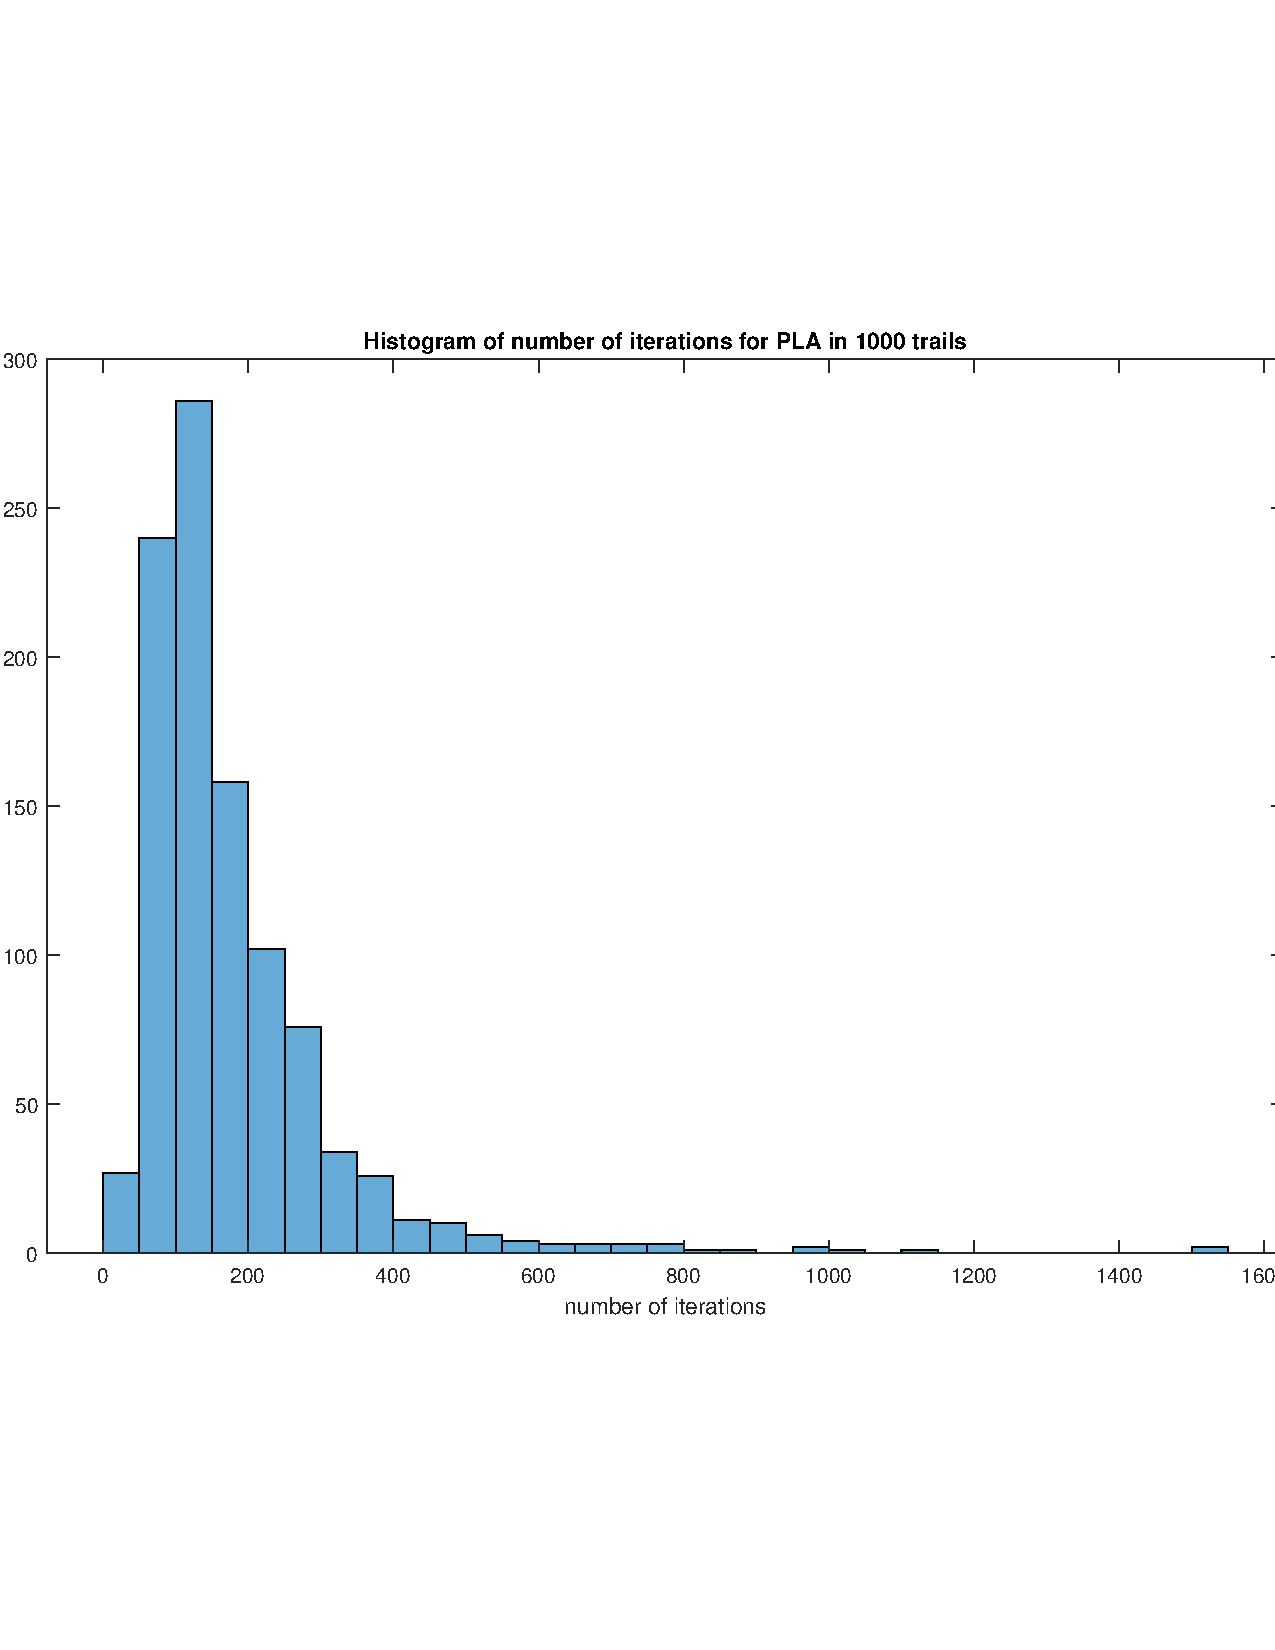
\includegraphics[width=6in]{prob2-1.pdf}
  \end{figure}
  
  \begin{figure}[H]
    \centering
    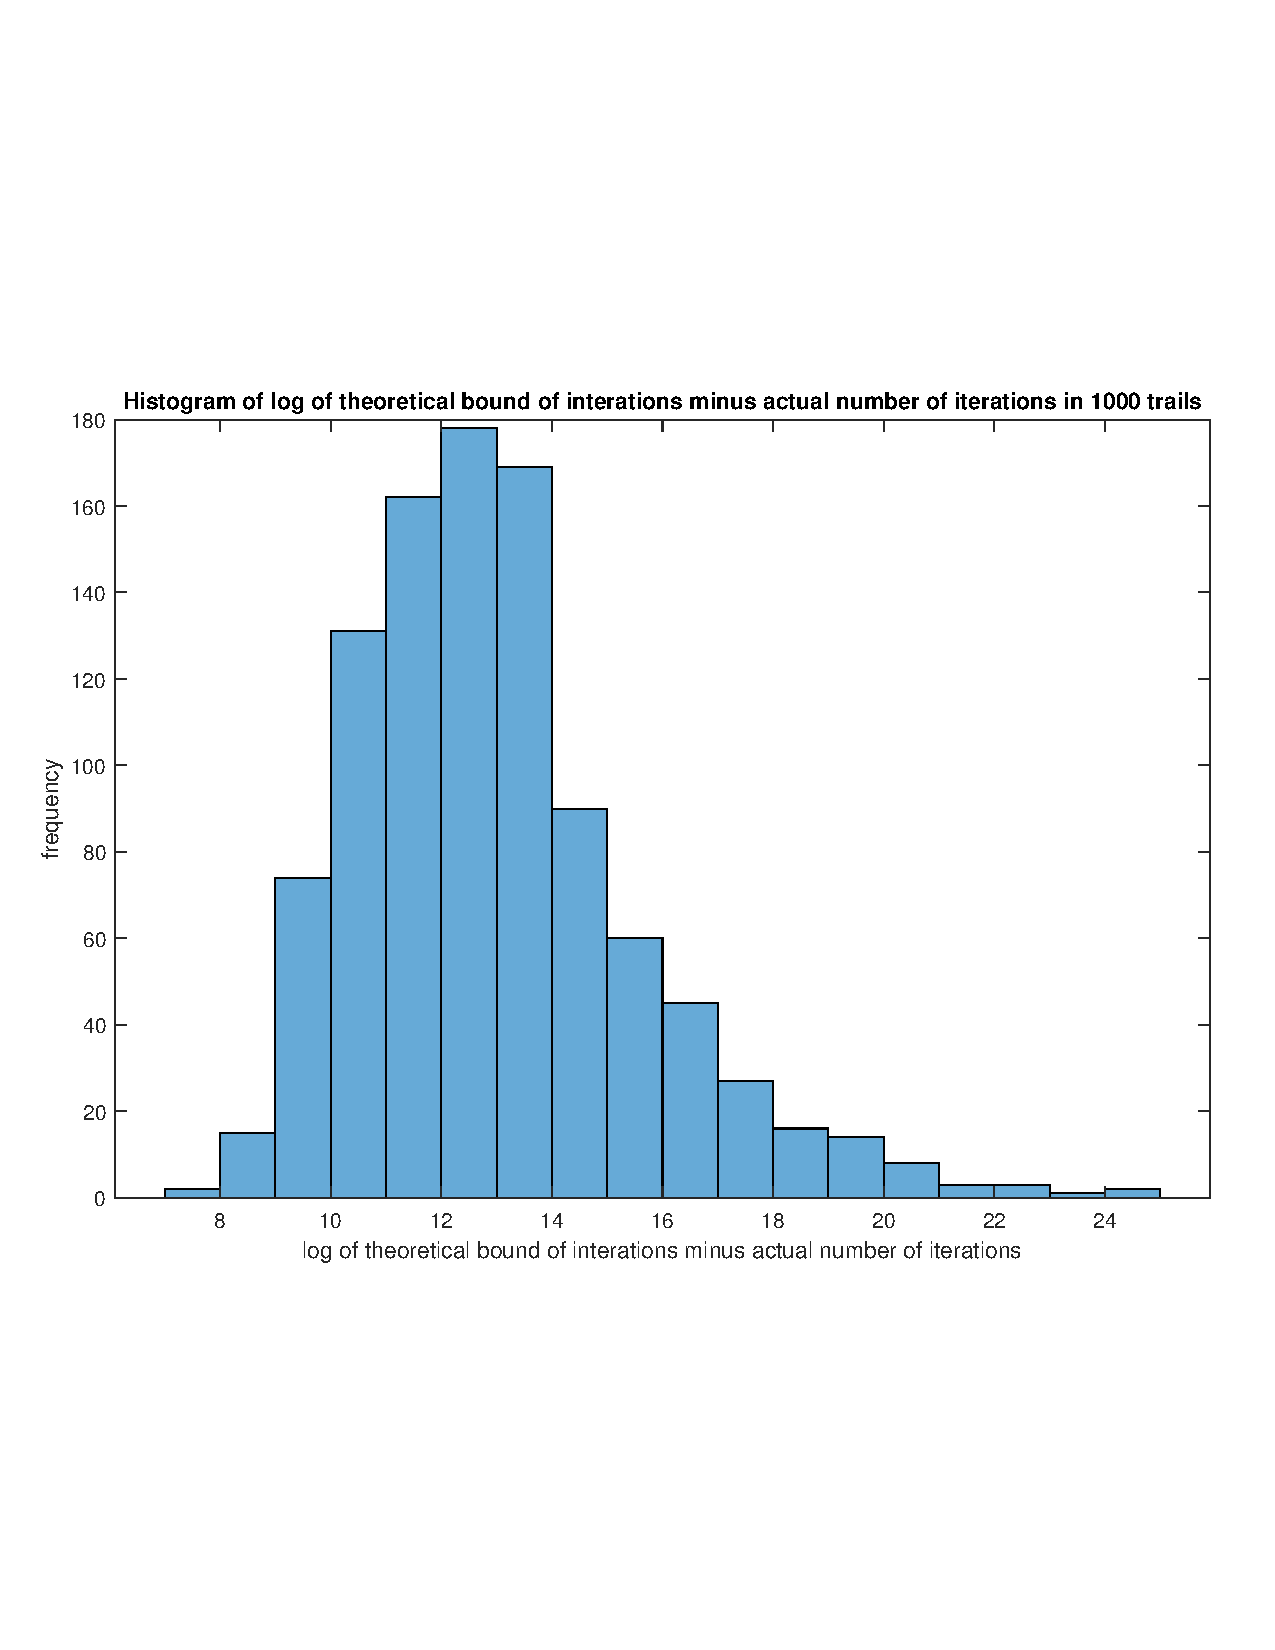
\includegraphics[width=7in]{prob2-2.pdf}
  \end{figure}

 The iterations of the PLA in 1000 trails looked approximately normal but with some right skew. The theoretical upper bound are mostly way larger than the steps it actually takes. 

 \item LFD problem 1.7
  \begin{enumerate}
    \item
    Set event E as at least one coin will have $\nu =0$, event F as no coin will have $\nu =0 $ and c denote number of coins
    \begin{itemize}
      \item when $\mu =0.05$:\\
      $\mathbb{P}(k=0,N=10,\mu=0.05)={10\choose 0}\cdot 0.05^0 \cdot (1-0.05)^{10-0} = 0.5987$ \\
       $\mathbb{P}(E|c=n) = 1-\mathbb{P}(F|c=n) \\ $ Because every coin follows a binomial distribution with p =0.5987 to get $\nu =0$ \\
       When n=1: $\mathbb{P}(E|c=n) = 1- (1-p)^n =0.5987 $ \\
       Similarly, when n=1,000: $\mathbb{P}(E|c=n) = 1- (1-p)^n =1 $ \\
       When n=1,000,000: $\mathbb{P}(E|c=n) = 1- (1-p)^n =1 $ \\
      \item $\mu =0.8$:\\
      $\mathbb{P}(k=0,N=10,\mu=0.8)= {10\choose0} \cdot 0.8^0 \cdot (1-0.8)^{10-0} = 1.024 \cdot 10^{-7}$ \\
      $\mathbb{P}(E|c=n) = 1-\mathbb{P}(F|c=n) \\ $ Because every coin follows a bernoulli distribution with $p =1.024 \cdot 10^{-7}$ to get $\nu =0$ \\
       When n=1: $\mathbb{P}(E|c=n) = 1- (1-p)^n = 1.024 \cdot 10^{-7} $ \\
       Similarly, when n=1,000: $\mathbb{P}(E|c=n) = 1- (1-p)^n =0.0001 $ \\
       When n=1,000,000: $\mathbb{P}(E|c=n) = 1- (1-p)^n =0.097 $ \\
    \end{itemize}
    \item
    Denote A as the event that $| \nu_1 -\mu|_1 > \epsilon$ and B as the event that $| \nu_2 -\mu_2| > \epsilon$ \\
    Then: \\ $\mathbb{P}(Max|\nu_i-\mu_i|> \epsilon) \leq \mathbb{P}(A or B) = \mathbb{P}(A)+\mathbb{P}(B)+ \mathbb{P}(A~ and~B)$ \\
    Because $\mathbb{P}(A~ and~B)$ always greater or equal to 0, we have:\\ $\mathbb{P}(Max|\nu_i-\mu_i|> \epsilon) \leq \mathbb{P}(A)+\mathbb{P}(B)$ \\
    Thus:\\  $\mathbb{P}(Max|\nu_i-\mu_i|> \epsilon) \leq 2\cdot 2e^{-2N\epsilon^2}=4e^{-12\epsilon^2}$
  \end{enumerate}
  
  
  \begin{figure}[H]
    \centering
    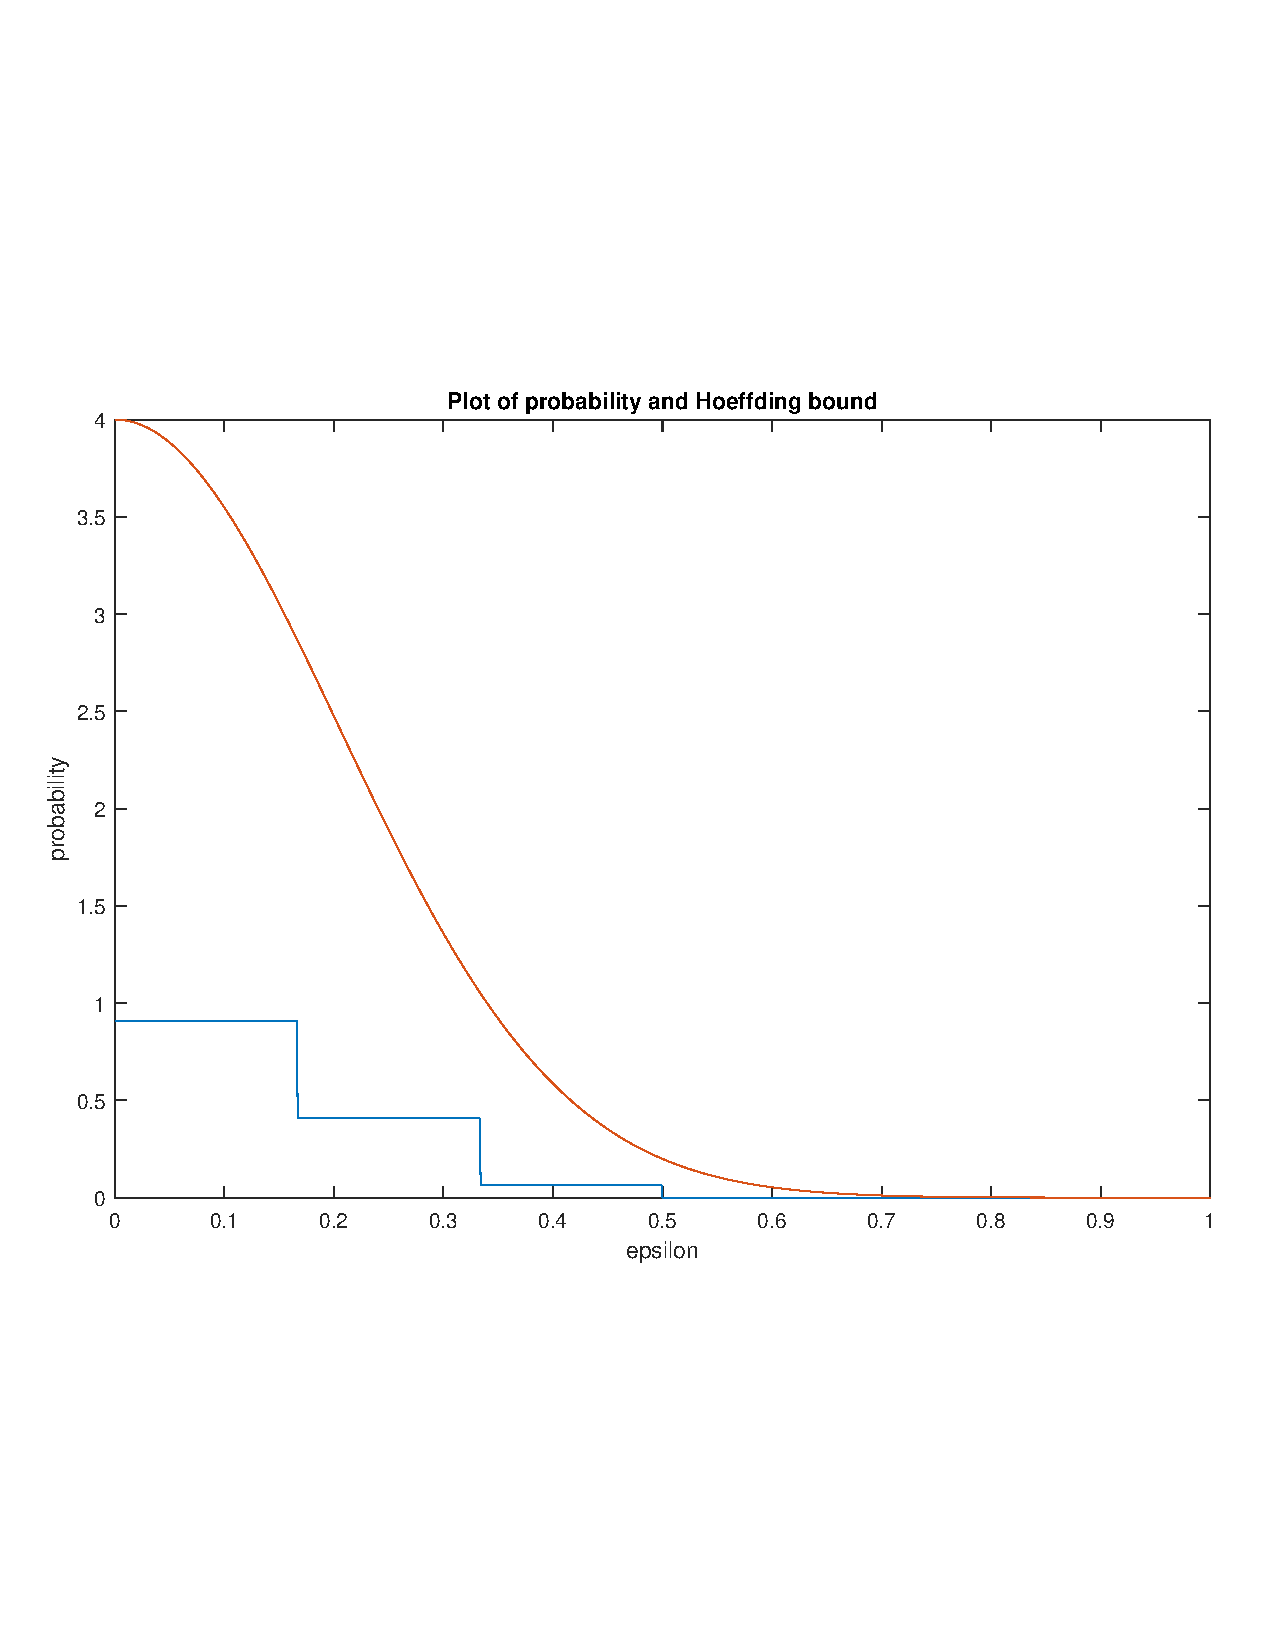
\includegraphics[width=7in]{prob3-2.pdf}
  \end{figure}

    \item LFD problem 1.8
    \begin{enumerate}
      \item
      \begin{proof}
        For a non-negative random variable $\alpha >0$ We can have a non-negative variable t that satisifys
      \begin{equation*}
        \alpha \mathbb{I}_{t \geq \alpha} \leq t
      \end{equation*}
      As when $t \geq \alpha$, $\alpha \cdot 1 \leq t$; when $t < \alpha$, $\alpha \cdot 0 \leq t$ \\
      Taking expectation on both sides we have:
      \begin{equation*}
      \begin{split}
          \mathbb{E}( \alpha \mathbb{I}_{t \geq \alpha})& \leq \mathbb{E}( t) \\
          \Leftrightarrow \alpha\cdot 1 \cdot\mathbb{P}(t\geq \alpha) + \alpha \cdot 0\cdot \mathbb{P}(t < \alpha) = \alpha \mathbb{P}(t \geq \alpha) & \leq \mathbb{E}(t) \\
         \Leftrightarrow \mathbb{P}(t \geq \alpha) & \leq \frac{\mathbb{E}(t)}{\alpha}
      \end{split}
      \end{equation*}
      \end{proof}

      \item
      \begin{proof}
        According to part a) we easily get that ($(u-\mu)^2 \geq 0 $):
      \begin{equation*}
        \mathbb{P}((u-\mu)^2 \geq \alpha) \leq \frac{\mathbb{E}((u-\mu)^2) }{\alpha}
      \end{equation*}
      Because u has a mean $\mu$ and variance $\sigma^2$; according to the definition of variance, we have:
      \begin{equation*}
        \mathbb{P}((u-\mu)^2 \geq \alpha) \leq \frac{\sigma^2 }{\alpha}
      \end{equation*}
      \end{proof}
      \item
      \begin{proof}
        Because $u=\frac{1}{N}\sum_{n=1}^{N}\mu$, According to the property of expected value and variance we have:
      \begin{equation*}
        \begin{split}
           \mathbb{E}(u) & =\frac{1}{N}\sum_{n=1}^{N}\mu =\mu  \\
             Var(u)& = \frac{1}{N}\sum_{n=1}^{N}\sigma^2 =\frac{\sigma^2}{N^2}
        \end{split}
      \end{equation*}
      Referring the conclusion of part b) we easily have:
      \begin{equation*}
        \mathbb{P}((u-\mu)^2 \geq \alpha) \leq \frac{\sigma^2 }{N\alpha}
      \end{equation*}

      \end{proof}

    \end{enumerate}

\end{enumerate}
 
 
\section{Appendix
}
\begin{appendices}
 \begin{lstlisting}
  function [ w iterations ] = perceptron_learn( data_in )

[nrow,ncol] = size(data_in);
true_label = data_in(1:nrow,ncol);
true_label = true_label';
w = zeros(1,ncol-1);
iterations = 0 ;
while isequal( sign(w*data_in(1:nrow, 1:ncol-1)'), true_label )==0
    index = find(sign(w*data_in(1:nrow, 1:ncol-1)')-true_label ~= 0);
    w = w+ data_in(index(1),ncol)*data_in(index(1),1:ncol-1);
    iterations = iterations+1;
end


end
  \end{lstlisting}

  \begin{lstlisting}
function [ num_iters bound_minus_ni] =
  perceptron_experiment ( N, d, num_samples )
num_iters = zeros(1,num_samples);
bounds = zeros(1,num_samples);
for i= 1:num_samples
    rng(i);

    w_star = rand(1,d+1);
    w_star(1)= 0;
    x = 2* rand(d+1,N)-1 ;
    x(1,1:N)= ones(1,N);
    correct_tag = sign(w_star*x);
    data_in = [x',correct_tag']; % nrow = N, ncol=d+2
    f =@precptron_learn;
    [w,iter] = perceptron_learn(data_in);
     num_iters(i)= iter;

    rho=min(correct_tag.*(w_star*x));           %from problem 1.3
    R2=max(sum(x.*x));
    W2=sum(w_star.*w_star);
    bounds(i)=R2*W2/rho^2;
    bound_minus_ni = bounds - num_iters

end
  \end{lstlisting}

  \begin{lstlisting}
  [c,d]= perceptron_experiment(100,10,1000)
    histogram(c);
    xlabel('number of iterations');
    ylabel('frequency');
    title('Histogram of number of iterations for PLA in 1000 trails')
    histogram(log(d));
    xlabel('log of theoretical bound of interations minus actual number of 
    iterations')
    ylabel('frequency')
     title('Histogram of log of theoretical bound of interations minus actual 
     number of iterations in 1000 trails')

  \end{lstlisting}
  \begin{lstlisting}
  function[proba probb] = max_abs(N,mu)

proba = zeros(1,1000);
probb = zeros(1,1000);
record = zeros(1,1000);
nnnn = 0;
for j = 1:1000
    epsilon = j/1000;

    for i = 1:1000
        rng(i);
        c1 = randi([0,1],1,N);
        nu1 = mean(c1);
        rng(i+1000);
        c2 = randi([0,1],1,N);
        nu2= mean(c2);
        m = max(abs(nu1-mu),abs(nu2-mu));
        record(i) = m > epsilon ;

    end

    proba(j) = mean(record);
    probb(j) = 4 * exp(-12 * epsilon^2);
    nnnn = nnnn+1
end

end


 [aa,bb] = max_abs(6,0.5)
 epsilon = (1:1000)/1000;
 plot(epsilon, aa, epsilon,bb)
 xlabel('epsilon')
 ylabel('probability')
 title('Plot of probability and Hoeffding bound')
  \end{lstlisting}

\end{appendices}
\end{document} 